\mode*

% Since this a solution template for a generic talk, very little can
% be said about how it should be structured. However, the talk length
% of between 15min and 45min and the theme suggest that you stick to
% the following rules:  

% - Exactly two or three sections (other than the summary).
% - At *most* three subsections per section.
% - Talk about 30s to 2min per frame. So there should be between about
%   15 and 30 frames, all told.


\section{The Big Picture}

\begin{frame}
  \begin{center}
    \textbf{Detection}
    \qquad
    \textbf{Prevention}
    \qquad
    Recovery
  \end{center}
\end{frame}

\begin{frame}
  \begin{definition}[Intrusion]
    \begin{itemize}
      \item event or combination of events that constitute a security incident, 
        where an intruder gains, or attempts to gain, access to a resource 
        without authorization.
    \end{itemize}
  \end{definition}

  \begin{definition}[Intrusion detection]
    \begin{itemize}
      \item service that monitors and analyzes system events to detect 
        intrusions.
    \end{itemize}
  \end{definition}
\end{frame}


\section{Intruders}

\begin{frame}
  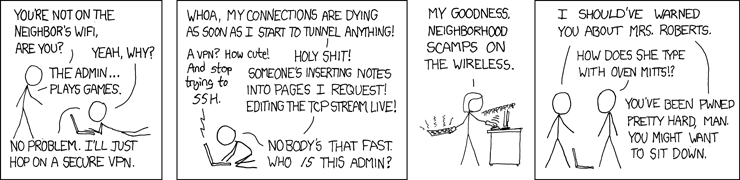
\includegraphics[width=\columnwidth]{figs/xkcd-341.png}
\end{frame}

\begin{frame}
  \begin{definition}[Intruders]
    \begin{description}
      \item[Masquerader] A user who is not authorized to use the system who 
        penetrates the access control of the system to exploit the user account 
        of a legitimate user.
        (Typically outsider.)

      \item[Misfeasor] A legitimate user who accesses resources for which such 
        access is not authorized, or who misuses his or her privileges.
        (Typically insider.)

      \item[Clandestine user] An individual who seizes supervisory control of 
        the system and uses this control to evade auditing or to suppress audit 
        collection.
    \end{description}
  \end{definition}
\end{frame}

\begin{frame}
  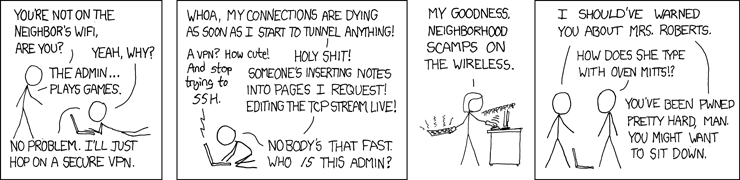
\includegraphics[width=\columnwidth]{figs/xkcd-341.png}
  \begin{example}
    \begin{itemize}
      \item The intruder above is a \emph{masquerader}.
      \item Mrs~Roberts' children are probably \emph{misfeasors}.
    \end{itemize}
  \end{example}
\end{frame}

\subsection{Behaviour Patterns}

\begin{frame}
  \begin{question}
    \begin{itemize}
      \item How does an intruder intrude?
    \end{itemize}
  \end{question}
\end{frame}

\begin{frame}
  \begin{example}[Ways to intrude]
    \begin{itemize}
      \item Phished user credentials
      \item Software bugs in access control
      \item Malware, combination of the previous two.
    \end{itemize}
  \end{example}
\end{frame}

\begin{frame}
  \begin{remark}
    \begin{itemize}
      \item The goal is different from that of ordinary users.
      \item Will this result in a change in behaviour?
    \end{itemize}
  \end{remark}
\end{frame}

\begin{frame}
  \begin{example}[\enquote{Hackers}]
    \begin{itemize}
      \item The \enquote{hacker} will look for targets of opportunities.
    \end{itemize}
  \end{example}

  \begin{definition}
    \begin{description}
      \item[White hat] A benign hacker who is exploratory in nature.
        Notifies targets of findings, bug-bounty hunter.

      \item[Black hat] A malicious hacker who tries to maximize his own gains.
    \end{description}
  \end{definition}
\end{frame}

\begin{frame}
  \begin{figure}
    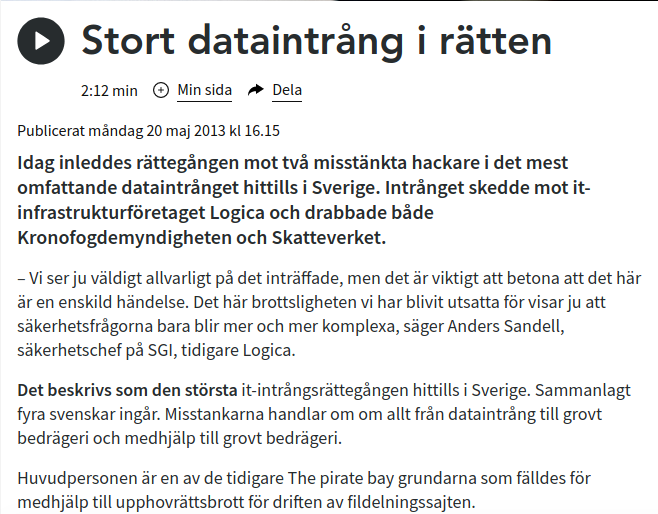
\includegraphics[width=\columnwidth]{figs/skatteverket-hack.png}
    \caption{\url{https://sverigesradio.se/artikel/5540019}}
  \end{figure}
\end{frame}

\begin{frame}
  \begin{example}[Criminal organizations]
    \begin{itemize}
      \item The criminal organisations will target specific systems of interest.
    \end{itemize}
  \end{example}

  \begin{example}[Randomware]
    \begin{itemize}
      \item Deploy software that encrypts as much vital data as possible.
    \end{itemize}
  \end{example}
\end{frame}

\begin{frame}
  \begin{figure}
    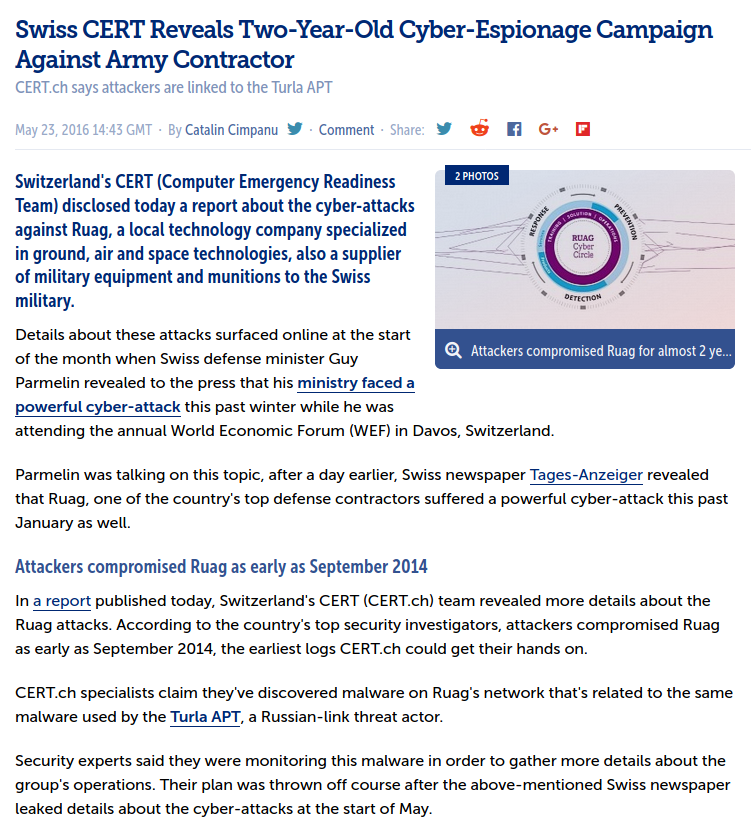
\includegraphics[width=\columnwidth]{figs/ruag-turla.png}
    \caption{\url{https://news.softpedia.com/news/swiss-cert-reveals-two-year-old-cyber-espionage-campaign-against-army-contractor-504385.shtml}}
    %\caption{\url{https://www.melani.admin.ch/dam/melani/en/dokumente/2016/technical\%20report\%20ruag.pdf.download.pdf/Report_Ruag-Espionage-Case.pdf}}
  \end{figure}
\end{frame}

\begin{frame}
  \begin{example}[Insider]
    \begin{itemize}
      \item The insider will just take information available to him or her.
      \item Counter by principle of least privilege, logs, strong 
        authentication, terminate former employees' accounts.
    \end{itemize}
  \end{example}
\end{frame}

\begin{frame}
  \begin{figure}
    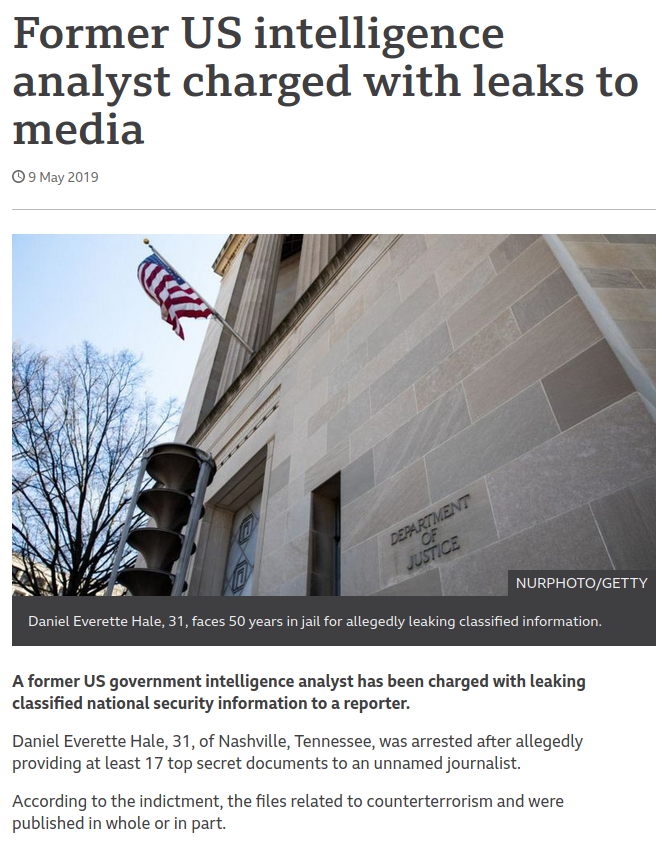
\includegraphics[width=\columnwidth]{figs/nsa-leak.png}
    \caption{\url{https://www.bbc.com/news/world-us-canada-48219097}}
  \end{figure}
\end{frame}

\begin{frame}
  \begin{figure}
    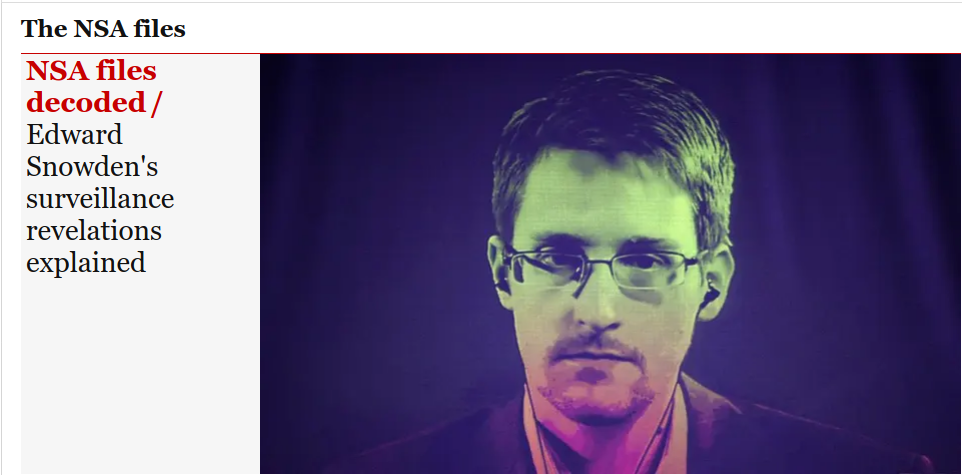
\includegraphics[width=\columnwidth]{figs/snowden.png}
    \caption{\url{https://www.theguardian.com/us-news/the-nsa-files}}
  \end{figure}
\end{frame}

%\subsection{Intrusion Techniques}
%
%\begin{frame}
%  \begin{enumerate}
%    \item Try default passwords with standard accounts.
%    \item Exhaustively try all short passwords.
%    \item Try a dictionary attack.
%    \item Collect information about the system users; \eg full names, names of 
%      spouses and children, pictures in their offices.
%    \item Try users' phone numbers, personal ID number, room numbers.
%    \item Try license plate numbers.
%    \item Use a Trojan horse to bypass restrictions on access.
%    \item Tap the connection between a remote user and the host system.
%  \end{enumerate}
%\end{frame}


\section{Intrusion Detection}

\begin{frame}
  \begin{question}
    \begin{itemize}
      \item How can we detect intruders?
    \end{itemize}
  \end{question}
\end{frame}

\begin{frame}
  \begin{idea}
    \begin{itemize}
      \item We can reasonably well distinguish masqueraders through past 
        history.

      \item Misfeasors can be detected by defining what's unauthorised use.

      \item Clandestine user is very difficult to detect automatically.
    \end{itemize}
  \end{idea}
\end{frame}

\begin{frame}
  \begin{remark}
    \begin{itemize}
      \item Intrusion detection is a difficult task.

      \item Based on the assumption that behaviour of intruder and legitimate 
        user can be quantified, and hence differences found.

      \item Problem is these behaviours might sometimes overlap.
    \end{itemize}
  \end{remark}
\end{frame}

\begin{frame}
  \begin{figure}
    \includegraphics[height=0.8\textheight]{figs/behaviour-profiles.pdf}
    \caption{Visualization of overlapping user behavioural profiles.}
  \end{figure}
\end{frame}

\begin{frame}
  \begin{example}[The problematic intersection]
    \begin{itemize}
      \item False positives: authorised users detected as intruders.
      \item False negatives: intruders detected as legitimate users.
    \end{itemize}
  \end{example}

  \pause

  \begin{remark}
    \begin{itemize}
      \item The base-rate fallacy!
    \end{itemize}
  \end{remark}
\end{frame}

\begin{frame}
  \begin{example}[Base-rate fallacy]
    \begin{itemize}
      \item Facial recognition software in airport.
      \item False negatives: if terrorist, alarm goes off 99/100.
      \item False positives: if non-terrorist, alarm goes off 1/100.
    \end{itemize}
  \end{example}

  \begin{exercise}[Base-rate fallacy]
    \begin{itemize}
      \item The alarm goes off, what's the probability that the person 
        scanned is a terrorist?
    \end{itemize}
  \end{exercise}
\end{frame}

\begin{frame}
  \begin{solution}[Base-rate fallacy]
    \begin{itemize}
      \item \(T\) means system indicates terrorist.
      \item We want to find \(\Pr(\terr\mid T)\):
        \only<1>{%
          \begin{align*}
            \Pr(\terr\mid T) &= \frac{\Pr(T\mid \terr) \Pr(\terr)}{\Pr(T)} \\
            \Pr(T\mid \terr) &= \frac{99}{100} \\
            \Pr(T\mid \lnot\terr) &= \frac{1}{100} \\
            \Pr(T) &= \Pr(T\mid \terr)\Pr(\terr) + \\
                   &\qquad\quad \Pr(T\mid \lnot\terr)(1-\Pr(\terr))
          \end{align*}
        }
        \only<2>{%
          \begin{align*}
            \Pr(\terr\mid T) &= \frac{\Pr(T\mid \terr) \Pr(\terr)}{\Pr(T)} \\
                             &= \frac{\frac{99}{100}\Pr(\terr)}{
                               \frac{99}{100}\Pr(\terr) +
                             \frac{1}{100}(1-\Pr(\terr))} \\
                             &= \frac{\frac{99}{100}\Pr(\terr)}{
                               \frac{98}{100}\Pr(\terr) +
                             \frac{1}{100}}
          \end{align*}
        }
    \end{itemize}
  \end{solution}
\end{frame}

\begin{frame}
  \begin{remark}
    \begin{itemize}
      \item How many terrorists are there?
      \item Assume that \(\Pr(\terr) = \frac{1}{1\,000\,000}\)\footnote{%
          30 hijackings per year (1978--2001), \(1.6\cdot 10^{9}\) passengers.
          Assume two terrorists per hijacked flight.
          %https://data.worldbank.org/indicator/IS.AIR.PSGR?end=2001&start=1978
          %https://ourworldindata.org/terrorism#airline-hijackings
        }.

        \pause

      \item That yields \(\Pr(\terr\mid T) \approx \frac{1}{10\,000}\).
      \item The alarm would be correct only \emph{once per 10\,000} alarms!
      \item Crying wolf?
    \end{itemize}
  \end{remark}
\end{frame}


\subsection{Where to collect data?}

\begin{frame}
  \begin{figure}
    \includegraphics[height=0.70\textheight]{figs/network-rotated.pdf}
    \caption{Example network topology.
      Two remote workers, one hacker and two servers connected over the 
      Internet.
      Three servers, four offices on the internal network.
    }
  \end{figure}
\end{frame}

\begin{frame}
  \centering
  \includegraphics[height=0.70\textheight]{figs/network-rotated.pdf}
  \begin{question}
    \begin{itemize}
      \item What data can we get if we place monitoring at the entrance?
    \end{itemize}
  \end{question}
\end{frame}

\begin{frame}
  \begin{figure}
    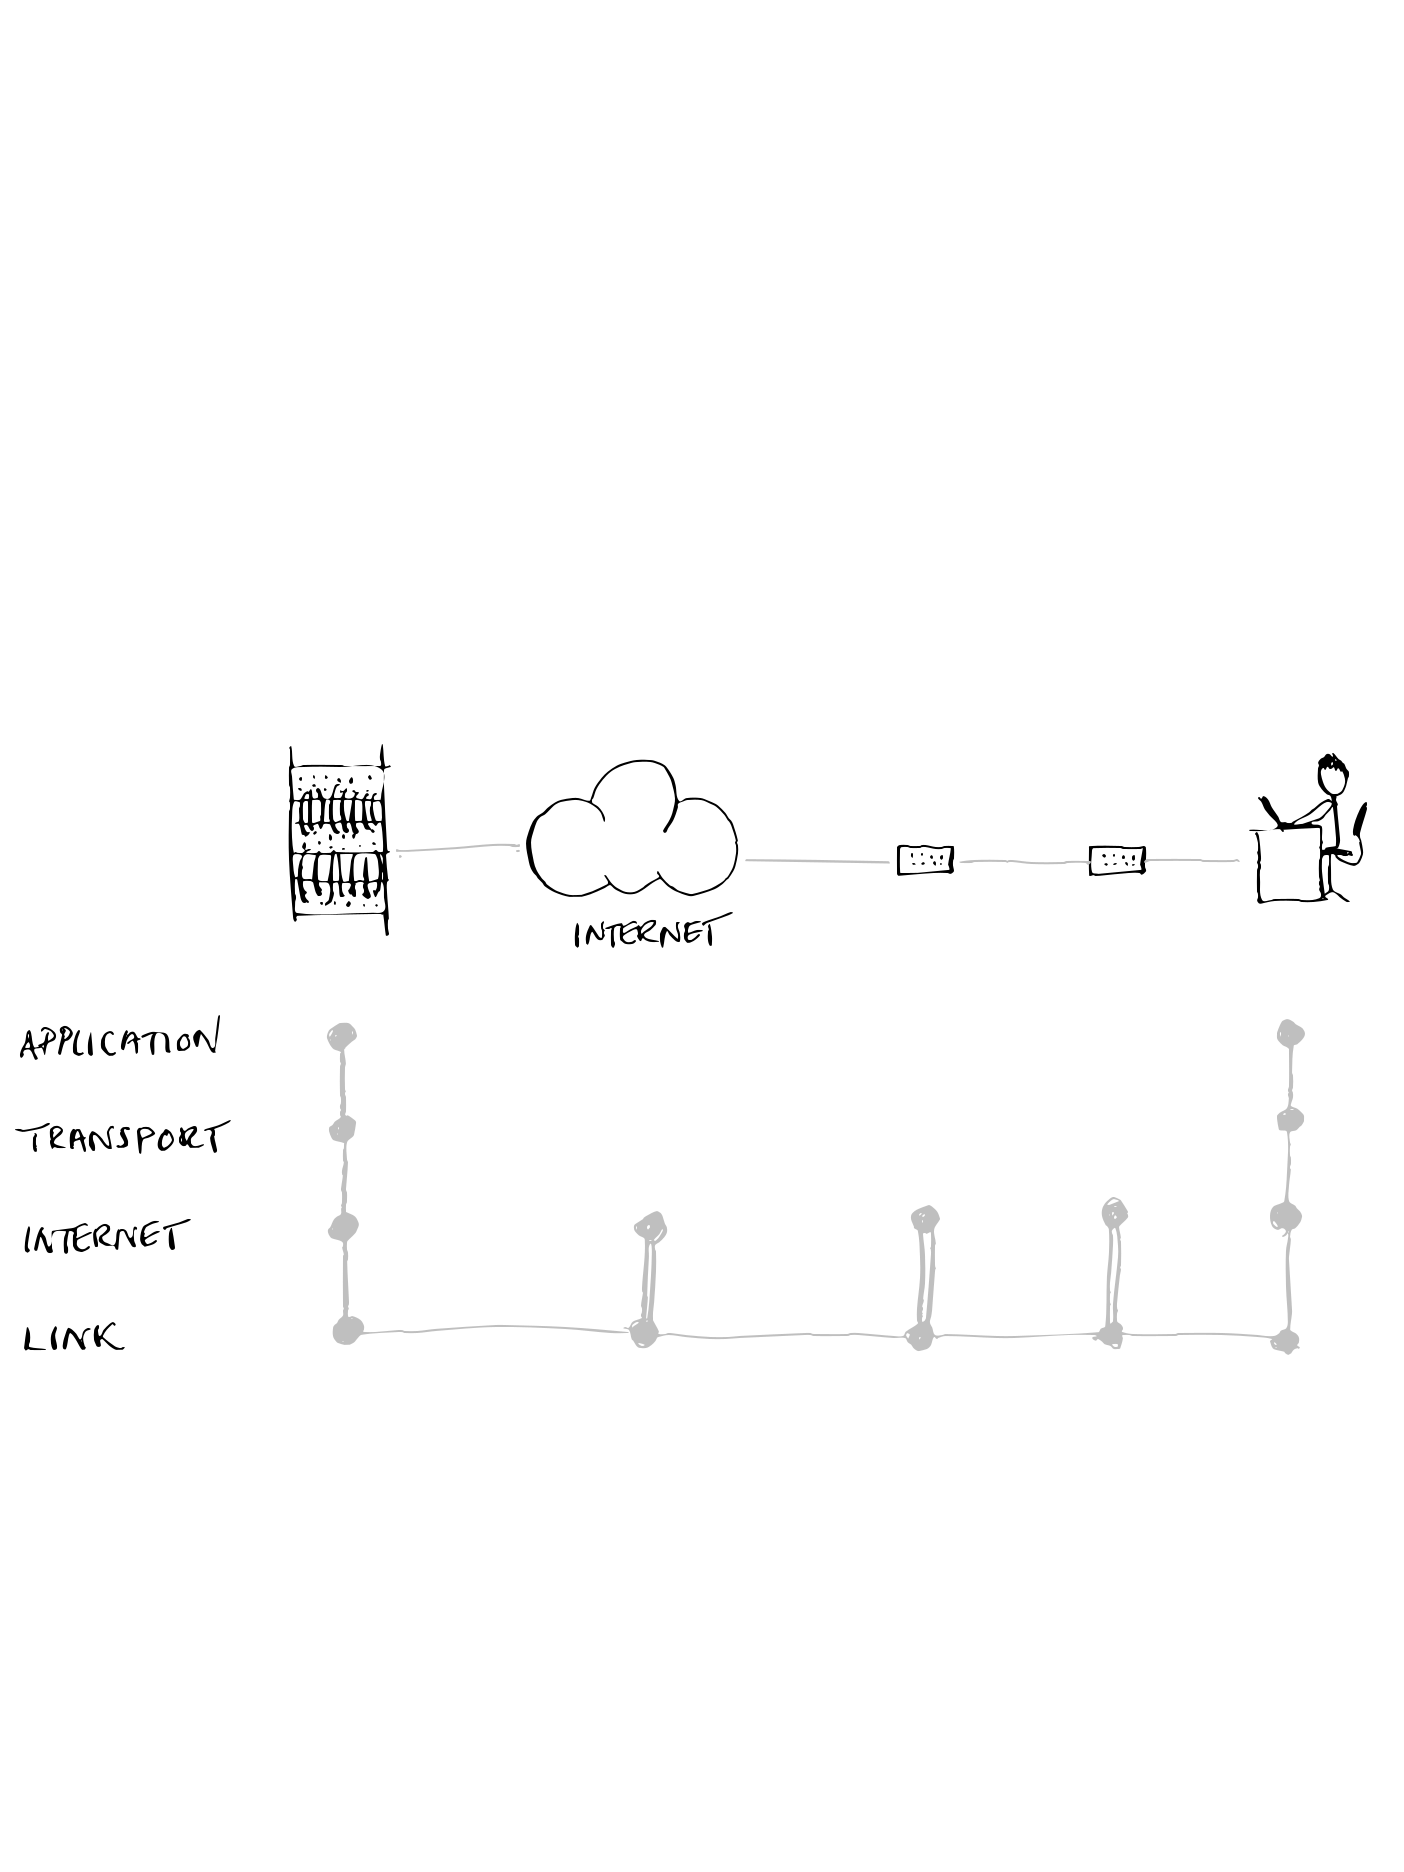
\includegraphics[height=0.7\textheight]{figs/network-layers.pdf}
    \caption{Communication between Bob and a server.}
  \end{figure}
\end{frame}

\begin{frame}
  \centering
  \includegraphics[height=0.60\textheight]{figs/network-rotated.pdf}

  \only<1>{
    \begin{definition}[Firewall]
      \begin{itemize}
        \item A firewall enforces certain traffic flows.
      \end{itemize}
    \end{definition}
  }
  \only<2>{
    \begin{example}[Firewall]
      \begin{itemize}
        \item Prevent outsiders from establishing connections to insiders.
        \item Insiders may establish connections to outsiders though.
      \end{itemize}
    \end{example}
  }
\end{frame}

\begin{frame}
  \centering
  \includegraphics[height=0.60\textheight]{figs/network-rotated.pdf}

  \only<1>{
    \begin{definition}[Network-based intrusion detection]
      \begin{itemize}
        \item Analyses events generated by network communication patterns.
        \item Internal and going outside.
      \end{itemize}
    \end{definition}
  }
  \only<2>{
    \begin{example}[Network-based intrusion detection]
      \begin{itemize}
        \item Connection from laptop to server.
        \item Immediately followed by connection to outside.
      \end{itemize}
    \end{example}
  }
\end{frame}

\begin{frame}
  \centering
  \includegraphics[height=0.70\textheight]{figs/network-rotated.pdf}
  \begin{question}
    \begin{itemize}
      \item What data can we get if we place monitoring at each server?
    \end{itemize}
  \end{question}
\end{frame}

\begin{frame}
  \begin{definition}[Host-based intrusion detection]
    \begin{itemize}
      \item Analyses events inside a host.
      \item Taps into the operating system.
    \end{itemize}
  \end{definition}

  \pause

  \begin{example}[Host-based intrusion detection]
    \begin{itemize}
      \item Rapid file reading, writing and deletion might indicate 
        ransonmware.
    \end{itemize}
  \end{example}
\end{frame}

\begin{frame}
  \begin{block}{Sensors and analysers}
    \begin{itemize}
      \item Sensors collect events data.
      \item Analysers analyses events data.
      \item Can be separate systems.
    \end{itemize}
  \end{block}
\end{frame}

\begin{frame}
  \begin{remark}[Audit records]
    \begin{itemize}
      \item Can use native audit records provided by OS.
      \item Can use custom for intrusion-detection system.
    \end{itemize}
  \end{remark}

  \pause

  \begin{example}[Logica/Skatteverket hack]
    \begin{itemize}
      \item Logica invoiced customers for CPU time.
      \item Intrusion (manually) detected by abnormally high invoice.
    \end{itemize}
  \end{example}
\end{frame}


\subsection{How to analyse data?}

\begin{frame}
  \begin{block}{Two approaches}
    \begin{description}
      \item[Signature based] Define rules of intruder behaviour.
      \item[Anomaly based] Learn normal behaviour, detect deviations.
    \end{description}
  \end{block}
\end{frame}

\begin{frame}
  \begin{definition}[Anomaly based]
    \begin{description}
      \item[Threshold] Define thresholds for various behaviours independently 
        of users.

      \item[Profile] Use a profile for each user to detect changes in behaviour.
    \end{description}
  \end{definition}
\end{frame}

\begin{frame}
  \begin{definition}[Signature based]
    \begin{itemize}
      \item Define rules for attack patterns (signatures).
    \end{itemize}
  \end{definition}

  \begin{example}[Signature based]
    \begin{itemize}
      \item Analyse attack scripts.
    \end{itemize}
  \end{example}
\end{frame}

\begin{frame}
  \begin{example}[Defence always behind]
    \begin{itemize}
      \item 54 days to patch, 6 days to exploit~\cite{SecurityEconometrics}.
    \end{itemize}
  \end{example}

  \begin{example}[Turla-APT's attack on RUAG]
    \begin{itemize}
      \item Did close to nothing \emph{first eight months!}
      \item Phoned home once per 90--180 days.
    \end{itemize}
  \end{example}
\end{frame}

\begin{frame}
  \begin{definition}[Honey pot]
    \begin{itemize}
      \item Decoy system.
      \item Has fabricated data.
      \item Any activity registered in that system is intruder activity.
    \end{itemize}
  \end{definition}
\end{frame}


\section{Summary}

\begin{frame}
  \begin{block}{Summary}
    \begin{itemize}
      \item Intrusion detection is hard.
      \item Base-rate fallacy, crying wolf!
      \item Attackers crawl under the radar.
    \end{itemize}
  \end{block}
\end{frame}
